\documentclass[compress]{beamer}
\usepackage[latin1]{inputenc}
\usepackage[T1]{fontenc}
\usepackage[francais]{babel}
\usepackage{graphicx}
\usepackage{amsmath}
\usepackage{caption}
\usepackage{fancyhdr}
\usepackage{fancybox}
\usepackage{xcolor}
\usepackage{color}
\usepackage{pgf,tikz}
\usepackage{rotating}
\usepackage{schemabloc}
\usepackage{caption}
\usepackage{graphicx}
\usepackage{graphics}
\usepackage{setspace}
\usepackage{booktabs}

\setbeamertemplate{navigation symbols}{}

%% http://mcclinews.free.fr/latex/beamergalerie/completsgalerie.html
\usetheme{CambridgeUS} %% default, Bergen, Boadilla,Madrid, AnnArbor, CambridgeUS, Pittsburgh, Rochester, Antibes, JuanLesPins, Montpellier, Berkeley, PaloAlto, Goettingen, Marburg, Hannover, Berlin, Ilmenau, Dresden, Darmstadt, Frankfurt, Singapore, Szeged, Copenhagen, Luebeck, Malmoe,Warsaw

%% http://mcclinews.free.fr/latex/beamergalerie/colorgalerie.html
%\usecolortheme{orchid} %% default (rouge), dolphin et whale (bleu), wolverine (jaune), crane (jaune rempli), orchid (bleu rempli), rose, 
%% albatross, beaver, beetle, crane, default, dolphin, dove, fly, lily, orchid, rose, seagull, seahorse, sidebartab, structure, whale, wolverine

\usefonttheme{serif} %% default, serif, professionalfonts, structurebold, structureitalicserif, structuresmallcapsserif

%% http://mcclinews.free.fr/latex/beamergalerie/innergalerie.html
\useinnertheme{rounded} %% default, circles, rectangles, rounded, inmargin 

%% http://mcclinews.free.fr/latex/beamergalerie/outerdetails.html
%\useoutertheme{default} %% default, infolines, miniframes, shadow, sidebar, smoothbars, smoothtree, split, tree, 

%\definecolor{bleugris}{rgb}{0.2,.0.4,0.5}

\definecolor{darkred}{rgb}{0.00,0.00,1.00}
\setbeamercolor{titre}{bg=darkred,fg=white}
\setbeamercolor{texte}{bg=darkred!10,fg=black}
%\beamerboxesdeclarecolorscheme{blocbleu}{blue}{yellow}

%\definecolor{darkred}{rgb}{1.00,0.00,0.00}
%\setbeamercolor{titre}{bg=darkred,fg=white}
%\setbeamercolor{texte}{bg=darkred!10,fg=black}
%%\beamerboxesdeclarecolorscheme{blocbleu}{red}{yellow}

%\definecolor{darkred}{rgb}{0.00,1.00,0.00}
%\setbeamercolor{titre}{bg=darkred,fg=white}
%\setbeamercolor{texte}{bg=darkred!10,fg=black}
%%\beamerboxesdeclarecolorscheme{blocbleu}{blue}{yellow}

\setbeamerfont{page number in head/foot}{size=\tiny}
\definecolor{bleugris}{rgb}{0.2,.0.4,0.5}
\setbeamertemplate{navigation symbols}{}
\usefonttheme[onlylarge]{structurebold}

\title[]{}
\subtitle[]{}
\institute[]{}
\author[\hspace*{1.25cm}\textbf{BE Robotique}\hspace*{3cm}]{}
\date[]{}

\begin{document}
\providecommand*{\figurename}{}
\renewcommand*{\figurename}{Fig}

\begin{frame}
%\begin{beamerboxesrounded}[upper=titre,lower=texte,shadow=true]{}
\centering
{{\textbf{Institut Sup�rieur d'Electronique de Paris}}} \\
%\vspace{0.5cm}

\includegraphics[scale=0.2]{ISEP.png} \\
%\vspace{3cm}
CT.1104 : BE Robotique \\
%\vspace{0.5cm}
{\large{\textbf{Robot NAO assistant dans un magasin}}} \\
%\vspace{1cm}
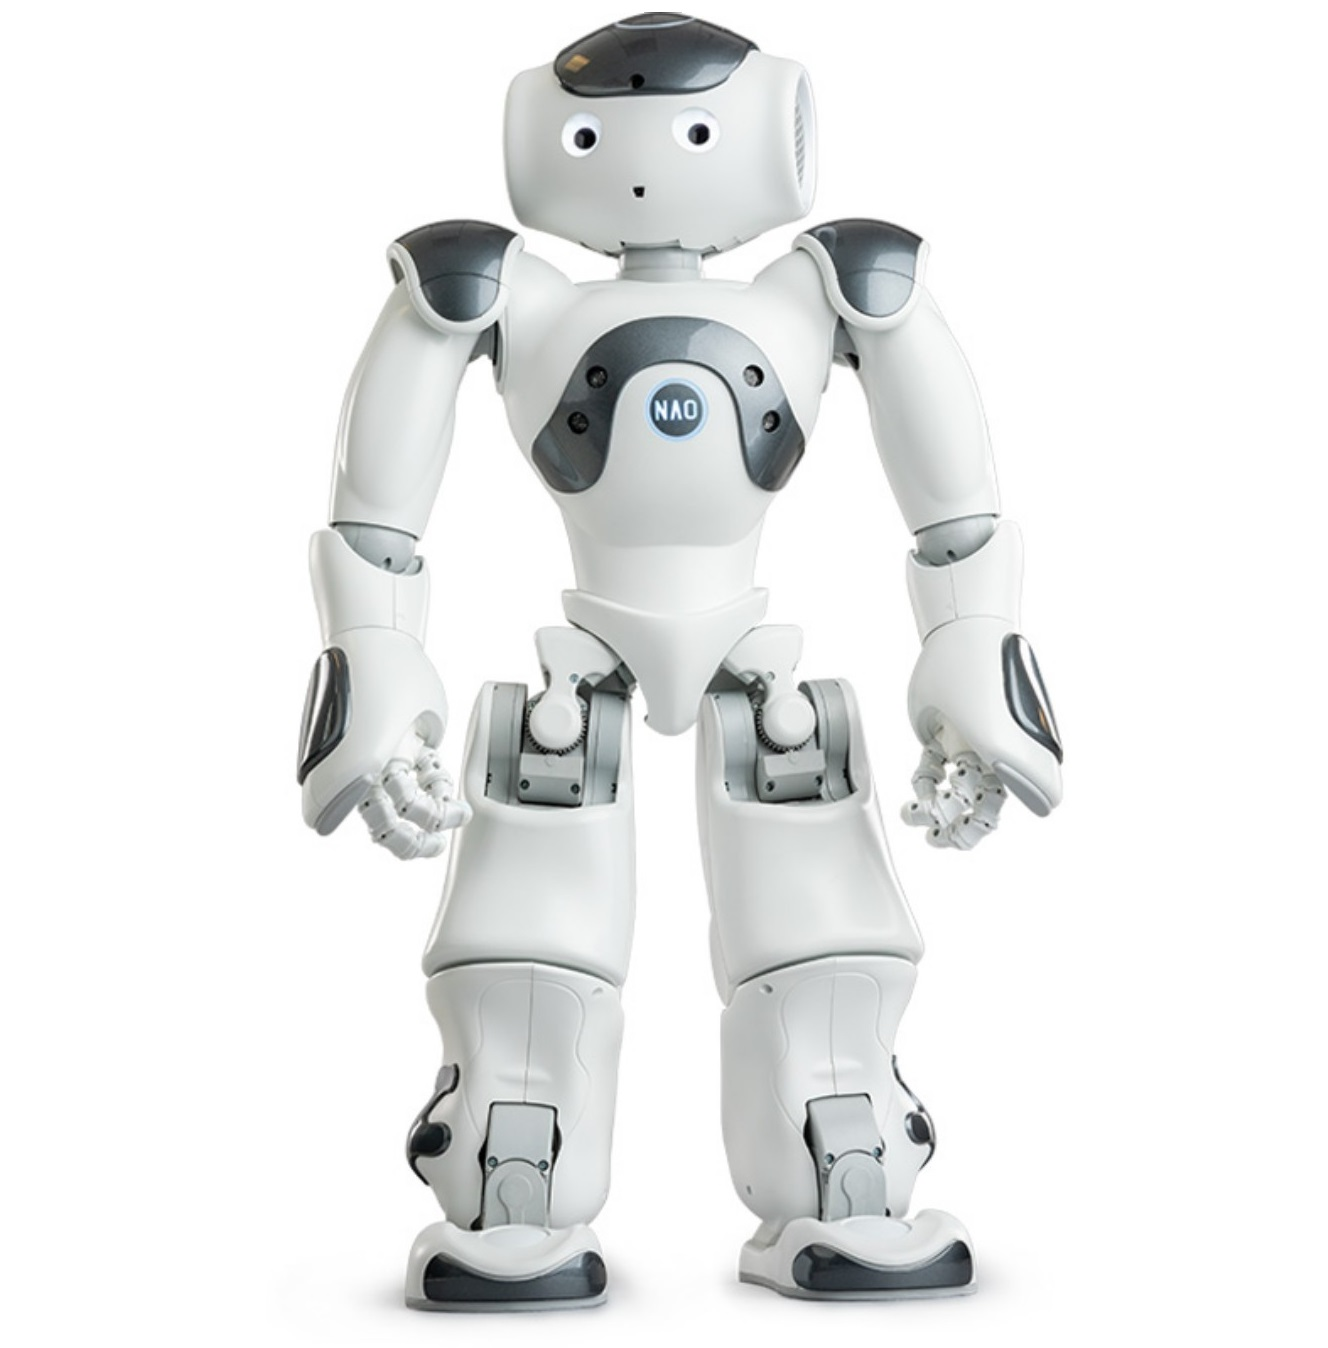
\includegraphics[scale=0.12]{NAO.jpg} \\
\vspace{-0.2cm}
\begin{table}
{\small{
\begin{tabular}{cll}
\textbf{Groupe ... :} & NOM Pr�nom, & NOM Pr�nom \\
 & NOM Pr�nom, & NOM Pr�nom \\
 & NOM Pr�nom, & NOM Pr�nom \\
\end{tabular}
}}
\end{table}
\vspace{-0.1cm}
{\footnotesize{\textbf{2021/2022}}}
%\end{beamerboxesrounded}
\end{frame}

\begin{frame}{Plan}
\transwipe[direction=0, duration=0.5]
\tableofcontents
\end{frame}

\section{\textbf{Introduction}}

\begin{frame}{Introduction}
\begin{beamerboxesrounded}[upper=titre,lower=texte,shadow=true]{\textbf{Le module CT.1104 : BE Robotique}}
\begin{itemize}
\item \textbf{Objectif :} projet de mise en \oe{}uvre du robot NAO. 
\item \textbf{D�marche :} sp�cifications, conception, d�veloppement, tests, int�gration, etc. 
\item \textbf{Curiosit� :} d�couvrir et comprendre les fonctionnalit�s du robot 
\item \textbf{Attention :} conserver son int�grit�. 
\end{itemize}
\end{beamerboxesrounded}
\end{frame}

\section{\textbf{Pr�sentation du robot}}

\begin{frame}{Pr�sentation du robot}
\begin{beamerboxesrounded}[upper=titre,lower=texte,shadow=true]{\textbf{Le robot NAO}}
\begin{itemize}
\item Robot humano�de.
\item 2006 : premi�re version publique du robot NAO. 
\item \texttt{Choregraphe} : logiciel de programmation du robot.
\item \textbf{Quelques caract�ristiques :} Poids : 5 $kg$. Longueur : 58 $cm$. 25 articulations.
\end{itemize}
\end{beamerboxesrounded}
\end{frame}

\begin{frame}{Pr�sentation du robot}
\begin{beamerboxesrounded}[upper=titre,lower=texte,shadow=true]{\textbf{Le robot NAO}}
\begin{center}
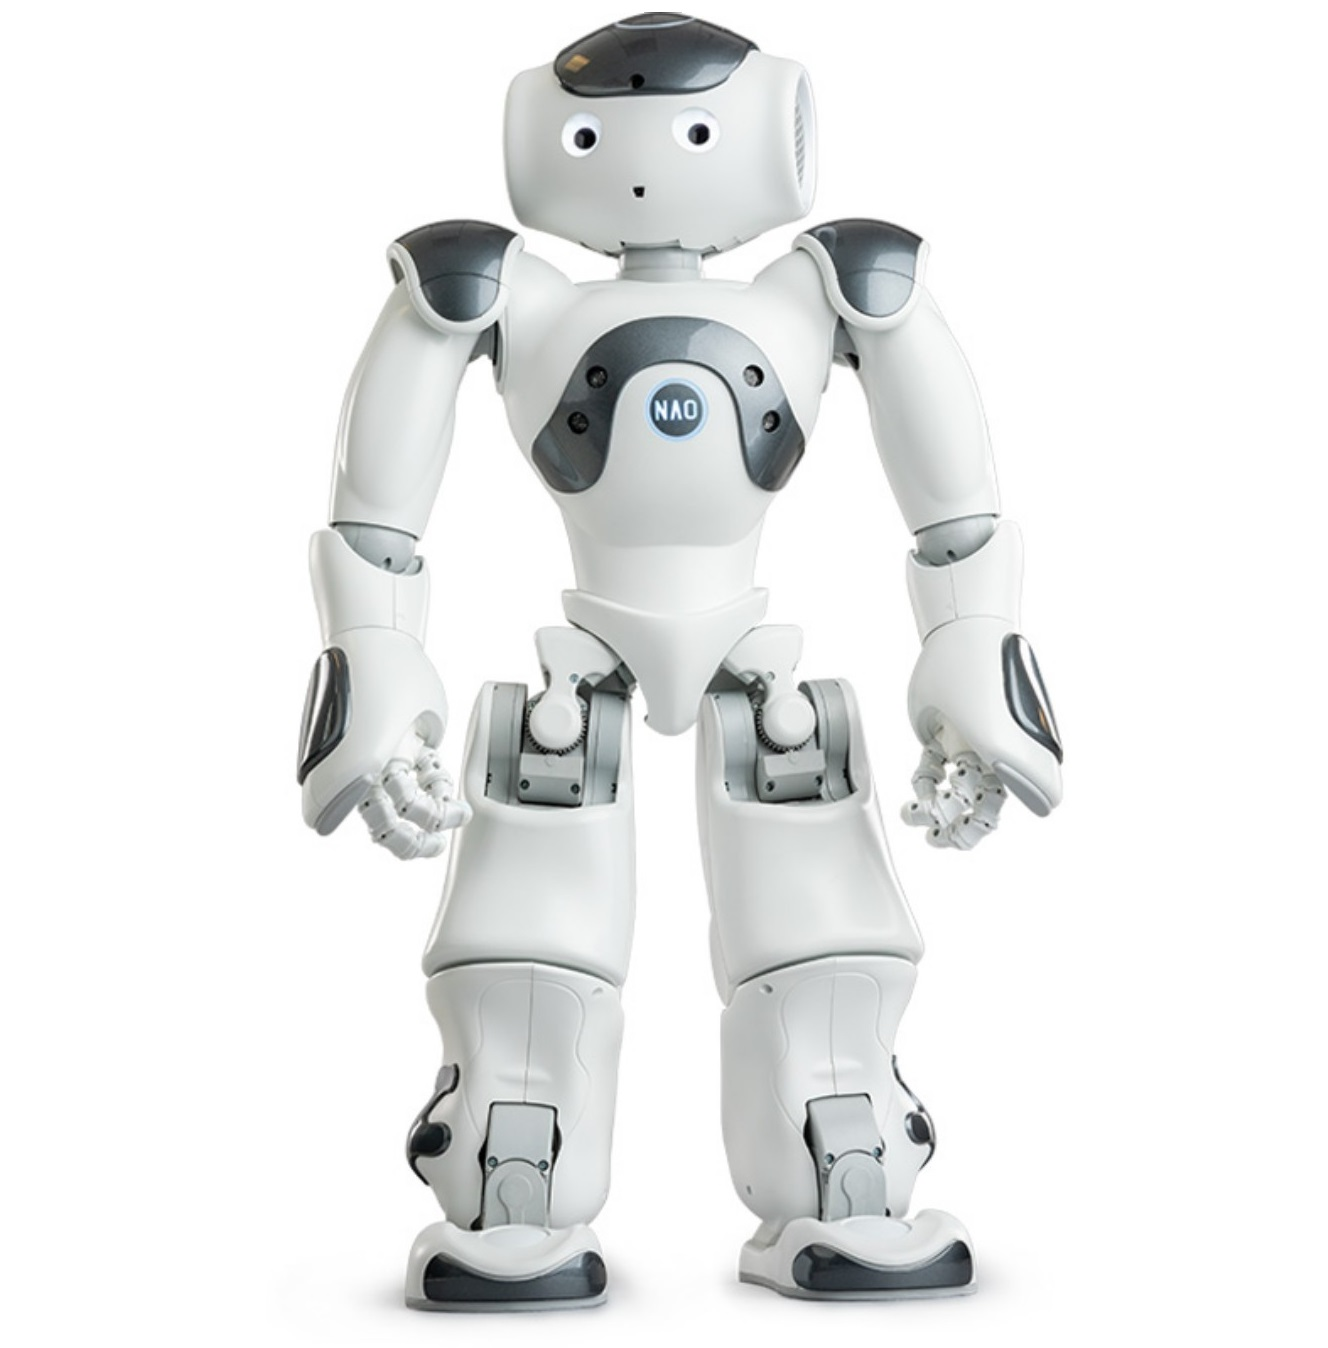
\includegraphics[scale=0.12]{NAO.jpg}
\captionof{figure}{Le robot NAO.}
\label{VP-6242G}
\end{center}
\end{beamerboxesrounded}
\end{frame}

\begin{frame}{Pr�sentation du robot}
\begin{beamerboxesrounded}[upper=titre,lower=texte,shadow=true]{\textbf{Param�tres de la convention DHM}}
\begin{table}[H]
\caption{Param�tres de la convention DHM correspondant au robot \texttt{Denso VP-6242G}.}
\centering
\begin{tabular}{c||c|c|c|c||c||c|c|c|c}
\toprule
\midrule
$i$ & $\alpha_i$ & $d_i$ & $r_i$ & $\theta_i$ & $i$ & $\alpha_i$ & $d_i$ & $r_i$ & $\theta_i$ \\
\midrule
\midrule
$1$ & $0$ & $0$ & $l_{1z}$ & $q_1$ & $4$ & $- \displaystyle \frac{\pi}{2}$ & $- l_{3x}$ & $l_{3z} + l_4$ & $q_4$ \\
\midrule
$2$ & $\displaystyle \frac{\pi}{2}$ & $0$ & $0$ & $q_2 + \displaystyle \frac{\pi}{2}$ & $5$ & $\displaystyle \frac{\pi}{2}$ & $0$ & $0$ & $q_5$ \\
\midrule
$3$ & $0$ & $l_2$ & $0$ & $q_3 - \displaystyle \frac{\pi}{2}$ & $6$ & $- \displaystyle \frac{\pi}{2}$ & $0$ & $l_5$ & $q_6$ \\
\midrule
\bottomrule
\end{tabular}
\label{tab:MDH}
\end{table}
\end{beamerboxesrounded}
\end{frame}

\begin{frame}{Pr�sentation du robot}
\begin{beamerboxesrounded}[upper=titre,lower=texte,shadow=true]{\textbf{Convention de Denavit-Hartenberg Modifi�e}}
\begin{figure}[H]
\begin{center}
%\resizebox{12cm}{!}{
\begin{tikzpicture}[scale=1]
\draw[black, ->,>=latex,very thick](0,0)--(0,5);
\draw[black, ->,>=latex,very thick](0,1)--(8,2);
\draw[black, ->,>=latex,very thick](6,1.75)--(4,6);
\draw[black, ->,>=latex,very thick](4.7,4.5)--(8,6);
\draw[red,dashed,>=latex,thick](6,1.75)--(6,4.3);
\draw[red,dashed,>=latex,thick](4.7,4.5)--(8.5,5);
\node(N1)at(3,1.35){\textcolor{blue}{$/$}};
\node(N1)at(6.9,4.75){\textcolor{blue}{$/$}};
\node(N1)at(0,3){\textcolor{blue}{$=$}};
\node(N1)at(6,3.5){\textcolor{blue}{$=$}};
\node(N1)at(-0.5,1.){$O_{i-1}$};
\node(N1)at(-0.6,2){$(R_{i-1})$};
\node(N1)at(4.4,4.5){$O_i$};
\node(N1)at(5.5,5.5){$(R_i)$};
\node(N1)at(8.4,1.9){$x_{i-1}$};
\node(N1)at(8.2,6){$x_i$};
\node(N1)at(0,5.2){$z_{i-1}$};
\node(N1)at(4,6.2){$z_i$};
\node(N1)at(2.6,1.55){$d_i$};
\node(N1)at(5.1,3.1){$r_i$};
\draw[->] (6,2.5) arc (0:160:0.18cm);
\draw[->] (5.75,4.6) arc (0:65:0.3cm);
\node(N1)at(5.75,2.85){$\alpha_i$};
\node(N1)at(6,4.8){$\theta_i$};
\end{tikzpicture}
%}
\end{center}
\end{figure}
\end{beamerboxesrounded}
\end{frame}

\begin{frame}{Pr�sentation du robot}
\begin{beamerboxesrounded}[upper=titre,lower=texte,shadow=true]{\textbf{Param�tres de la convention DHM}}
\begin{equation}
\left\{
\begin{array}{l}
\alpha_i = \widehat{z_{i-1},z_i} /x_{i-1} \\
d_i = \overline{O_{i-1},z_i} / x_{i-1} \\
r_i = \overline{x_{i-1},O_i} / z_i \\
\theta_i = \widehat{x_{i-1},x_i} /z_i \\
\end{array}
\right.
\label{DH}
\end{equation}
\end{beamerboxesrounded}
\end{frame}

\section{}

\begin{frame}{}
\begin{beamerboxesrounded}[upper=titre,lower=texte,shadow=true]{}
\begin{center}
{\fontsize{50}{1}\selectfont \textcolor{darkred}{\textbf{{{\fontfamily{pzc}\selectfont Merci pour votre attention}}}}}
\end{center}
\end{beamerboxesrounded}
\end{frame}

\end{document}

